 \documentclass[a4paper,10pt]{article}
 \usepackage[utf8]{inputenc}  
 \usepackage[T1]{fontenc}
 \usepackage{graphicx}
 \graphicspath{{images/}} 
 
 \usepackage{wrapfig} 
 \usepackage{amsmath} 
 \usepackage{gensymb}
 \usepackage{fancyhdr}
 \usepackage{lastpage}
 \usepackage{textcomp}
 \usepackage{color}
 \usepackage{colortbl}
 \usepackage[table]{xcolor}
 \usepackage{courier}
 \usepackage{setspace}
 \usepackage{listings}
 \usepackage{ulem}%
 \usepackage{geometry}
 \usepackage{array}
 \geometry{a4paper,
 total = {140mm, 237mm},
 left = 35mm,
 top = 30mm}
 \newcommand{\minus}{\scalebox{0.6}[1.0]{$-$}} 
 \newcommand{\signature}[2]{%
  \par\nobreak\bigskip
  \begin{singlespace}%
  \mbox{}\hfill\begin{tabular}{p{8cm} }
      \rule{8cm}{0.5pt}\newline{}%
        \textbf{#1}\\%
       #2 %
  \end{tabular}%
  \end{singlespace}%
  \medskip%
 }
 \renewcommand{\lstlistingname}{Extrait de code}
 \lstset{
 language=Java,
 basicstyle=\scriptsize\ttfamily, 
 upquote=true,
 aboveskip={1.5\baselineskip},
 columns=fullflexible,
 showstringspaces=false,
 extendedchars=true,
 frame=single,
 breaklines=true,
 showtabs=false,
 showspaces=false,
 showstringspaces=false,
 identifierstyle=\ttfamily,
 keywordstyle=\color[rgb]{0.2,0.2,0.2},
 commentstyle=\color[rgb]{0.133,0.545,0.133},
 stringstyle=\color[rgb]{0.627,0.126,0.941},
 tabsize=5,
 }
 \pagestyle{fancy}
 \fancyhead[R]{Projet final SigmaPi}
 \fancyfoot[C]{\thepage}
 \fancyhead[L]{Loïc Gillioz, Loïc Fracheboud}
 \author{Loïc Gillioz, Loïc Fracheboud}
 \title{Informatique - Projet final \\ \Huge SigmaPi (Patapon-like)}
 \date{13 juin 2016}
 \begin{document}
 \maketitle
 \begin{figure}[!h]
 \centering

 
\includegraphics[scale=0.15]{images/icones}
 \end{figure}
 \begin{figure}[!h]
 \centering
 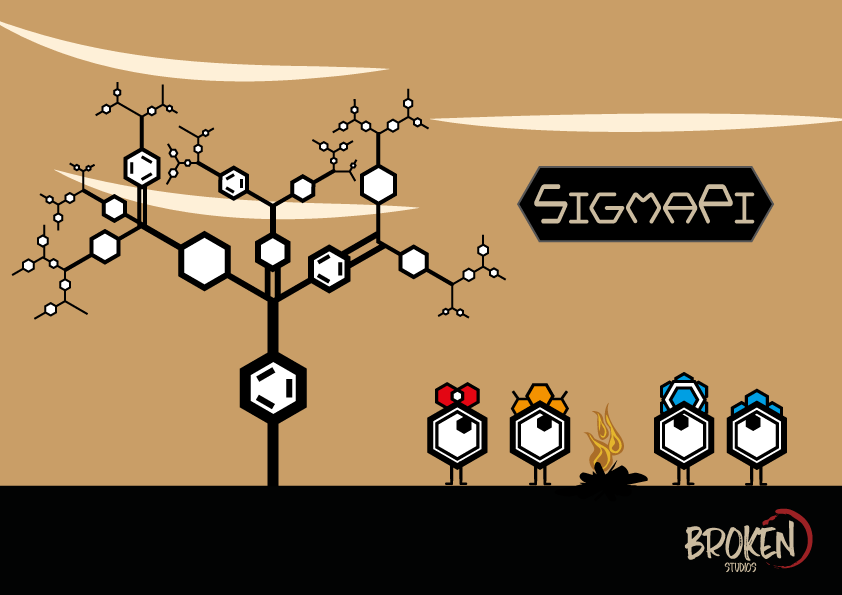
\includegraphics[scale=0.5]{images/couverture}
 \end{figure}
 \pagebreak
 
 \section{Description sommaire du jeu}
  SigmaPi est basé sur le jeu sorti sur PSP "Patapon". Ce jeu connu un grand succès et c'est désormais une des références des jeux de rythme. On y contrôle un groupe de personnages par le biais de quatre tambours en entrant des séquences (par exemple 3x carré puis 1x rond donne l'ordre d'avancer). On doit donc traverser des niveaux 2D à l'aide d'un nombre restreint de séquences.

  \paragraph{Github}
  Afin de gérer au mieux les versions de notre code, nous avons utilisé les fonctions de github. Vous pouvez donc retrouver tout l'historique de développement et tout le code à cette adresse : {\itshape https://github.com/loicfracheboud/SigmaPi}
  \begin{figure}[!h]
 \centering
 \vspace{5pt}
 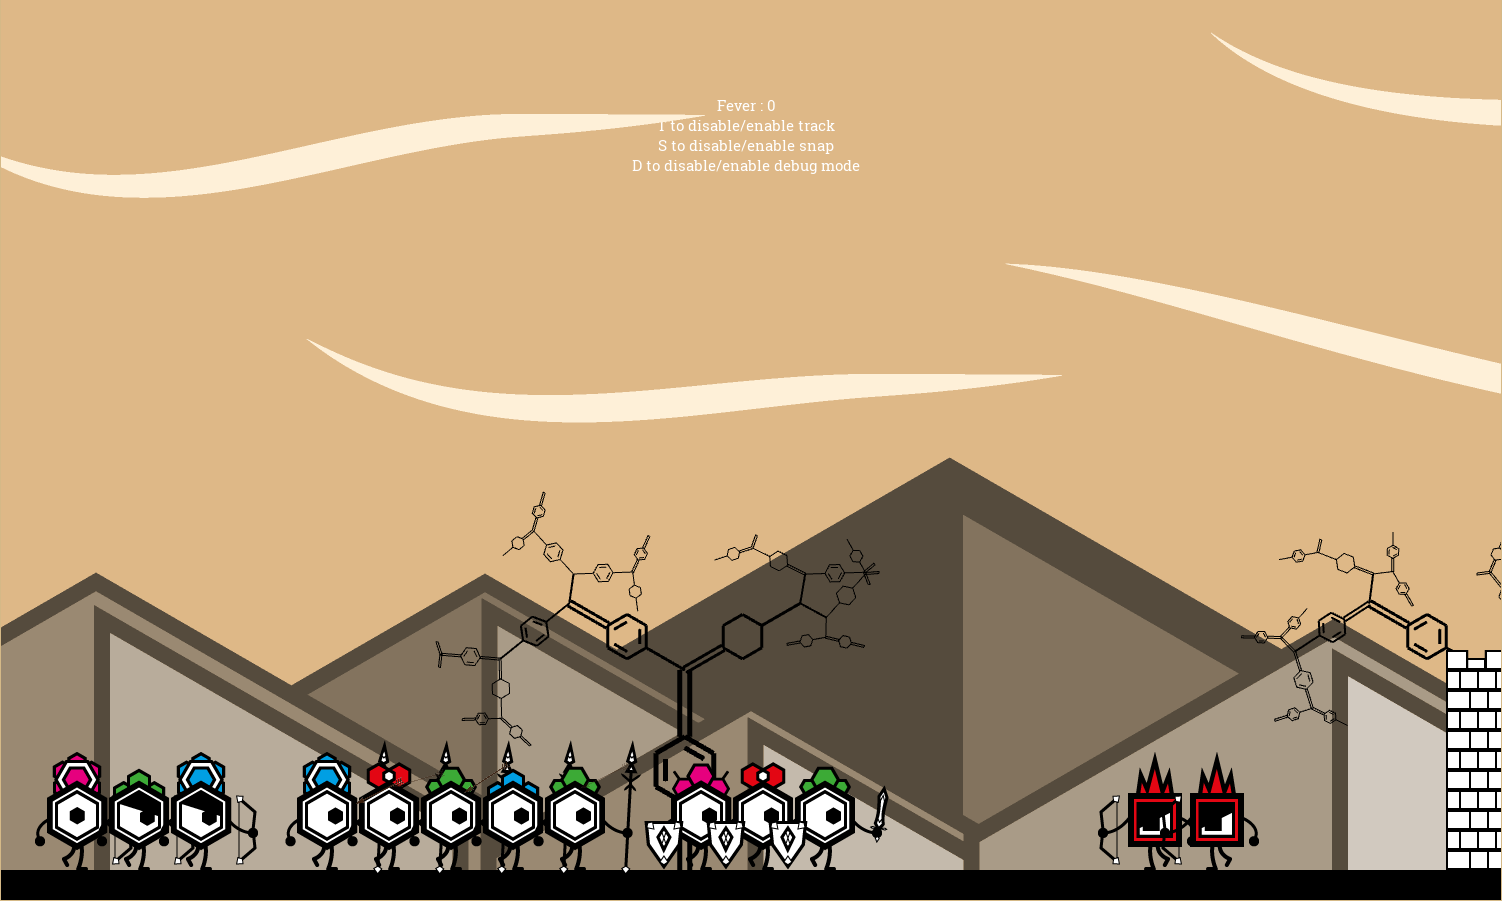
\includegraphics[scale=0.25]{images/menu}
 \caption{A gauche la compagnie du joueur et à droite deux archers ennemis}
 \end{figure}  
  \pagebreak
  
  \paragraph*{Structure UML}
  Comme on peut le voir sur la figure suivante, l'architecture du jeux est assez riche. On peut distinguer plusieurs groupes dédiés à des tâches communes, graphismes, mécanique de jeux, etc. INSERT UML
  \newline La structure du projet est composée de six packages différents :\begin{itemize}
  \item {\itshape drawable}
  \item {\itshape mechanics}
  \item {\itshape menus}
  \item {\itshape music}
  \item {\itshape physics}
  \item {\itshape units}
  \end{itemize}
  \paragraph{drawable}
  Ici nous avons toutes les classes qui s'occupent de la partie graphique du jeu, par exemple la classe SpriteSheet qui permet d'initialiser et travailler facilement avec les spritesheets.
 \begin{figure}[!h]
 \centering
 \vspace{-45pt}
 
\includegraphics[scale=0.3]{images/legs}
 \caption{Spritesheet des jambes des SigmaPi}
 \end{figure}
  \paragraph{mechanics}
  Ce package est axé sur la mécanique du jeu, c'est-à-dire gérer l'état des unités, instancier un niveau (les unités adverses et du joueur, etc).
  \paragraph{menus}
  Les différentes classes de ce niveau servent à générer des menus permettants de modifier les options du jeux, lancer une partie, etc. Pour l'instant nous n'avons pas implémenté ces fonctions, elles ne sont pas fondamentales.
  \paragraph{music}
  Toute la gestion des séquences entrées par le joueur est traitée ici (reconnaissance).
  \paragraph{physics}
  La physique est utile à plusieurs fonctions du jeu, notamment pour les flèches/lances et les hitboxes des unités.
  \paragraph{units}
  Ici nous avons toutes les classes qui s'occupent de la partie graphique du jeu, par exemple la classe SpriteSheet qui permet d'initialiser et travailler facilement avec les spritesheets.
  
  \pagebreak 
  \section{Architecture}
  Eclaircissons quelques points intéréssants du fonctionnement du jeu.
  \paragraph{Intelligence artificielle (AI)}
  Dans le jeu il y a deux types d'AI. La plus évidente est celle des adversaires. Lors d'une partie, ils sont créés et placés à une position x dans le niveau. Lorsque le joueur s'en approchera suffisamment, ils vont devenir agressifs et attaquer. Sachant que chaque unité à une certaine portée, ils vont se déplacer dans une zone définie afin de pouvoir nous atteindre.
  \newline Pour le joueur il existe un système similaire. C'est-à-dire que ses unités possèdent aussi une zone dans laquelle elle peuvent se déplacer pour faire correspondre leur portée à la position de la victime. La différence par rapport aux unités gérées par le jeu c'est que leur zone d'action bouge en fonction des actions du joueur.
  \newline Le deuxième point intéressant qui ne concerne que le joueur, c'est la faculté des unités à se regrouper selon un ordre bien défini lors des déplacements.
  \newline Tout ceci est possible grâce à une série de calculs determinants les déplacements potentiels et leur conséquences. En fonction de cela (et de la volonté du joueur), le système donne les instructions finales.
  
  \paragraph{Arbres récursifs}
  Dans le jeu on peut voir des arbres se mouvants au gré d'un vent parfaitement inexistant. Ces arbres sont générés avec les principes de récursivité et un peu de hasard. Nous avons défini quelques motifs de base (ligne simple/double, hexagone vide/rempli, etc) et quelques règles (chaque section est composée d'un élément ligne, puis un élément hexagone et à nouveau une ligne ou juste un élément ligne seul). A partir de là on peut générer un arbre.
 \begin{figure}[!h]
 \centering
 \vspace{-10pt}
 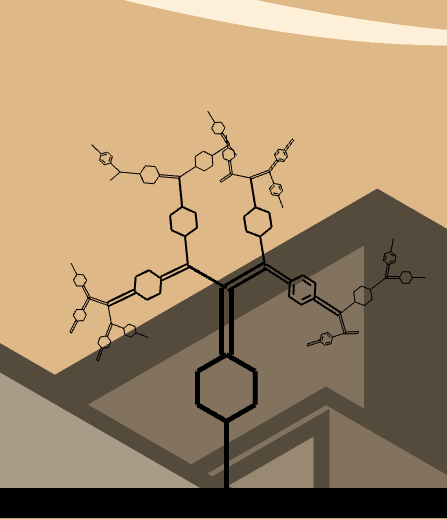
\includegraphics[scale=0.4]{images/tree}
 \caption{Exemple d'arbre, niveau de récursivité V}
 \end{figure}
  \newline Dans la classe de gestion du décors on peut donc appeler cette fonction de dessin d'arbre pour en faire une forêt. Dans notre cas, une forêt représente l'ensemble des arbres présents sur le niveau. La génération d'une forêt prend quelques paramètres en entrée et génère ensuite le nombre d'arbre désirés, avec une taille et un niveau de récursivité moyens afin d'avoir un résultat cohérent visuellement.
  \newline Reprenons l'arbre de la section précédente et comparons le à son voisin. On voit qu'ils ont le même niveau de récurivité, mais pas la même taille, ni la même structure.
 \begin{figure}[!h]
 \centering
 \vspace{-10pt}
 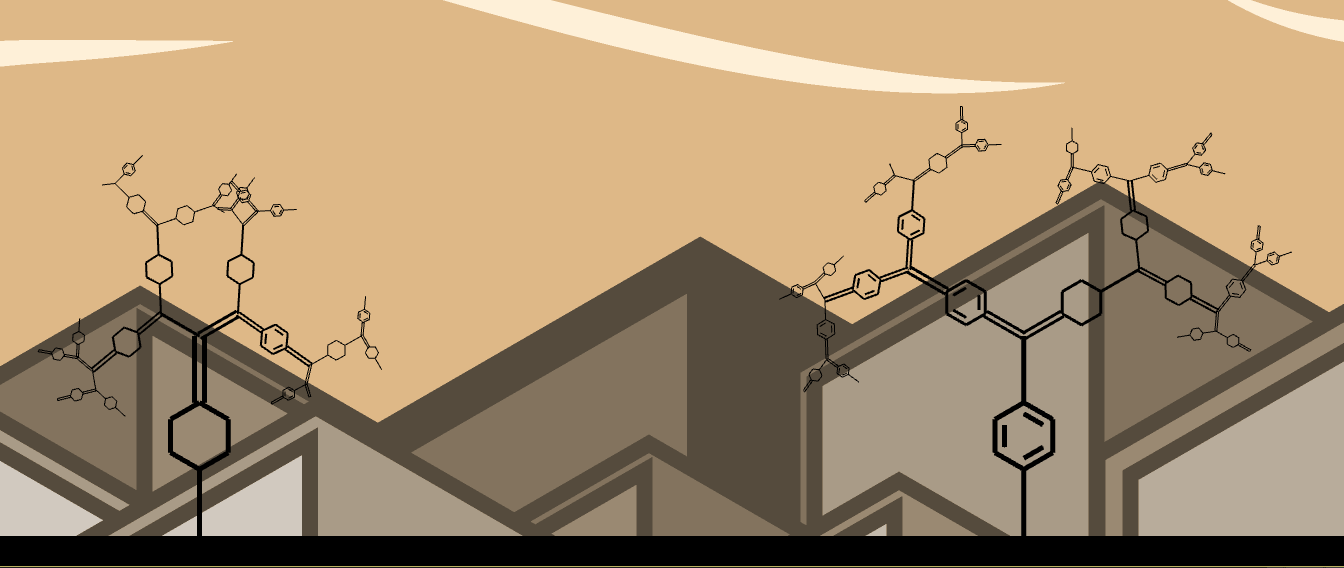
\includegraphics[scale=0.3]{images/trees}
 \caption{Deux arbres générés par le jeu}
 \end{figure}
  
  \pagebreak 
  \section{Confrontation au planning}
  Maintenant que le projet est terminé, nous pouvons tirer un bilan sur le planning prévu et celui réalisé. Pour rappel, nous avions planifié le travail comme suit :
  \paragraph{}
 \newcolumntype{M}[1]{>{\raggedright}m{#1}}
 {\rowcolors{1}{lightgray}{white}
\begin{tabular}{M{9cm}lc}
\bf Fonctionnalité & \bf  Date & \bf Importance \tabularnewline
Gestion des séquences de notes & Implémenté & +++ \tabularnewline
Gestion des actions par fonction (p.ex. les archers tirent des flèches, lanciers des lances, les épéistes frappent mais ne lancent rien) & 06.05.2016 & +++ \tabularnewline
    Déplacement de la caméra selon la position des SigmaPis & 12.05.2016  & +++\tabularnewline
    Utilisation de la physique pour les objets balistiques et des collisions & 20.05.2016 & ++ \tabularnewline
    Utilisation des collisions pour appliquer les dégâts aux unités & 20.05.2016 & ++\tabularnewline
    Adaptation des aptitudes des SigmaPis selon leur niveau et race & 12.06.2016 & ++\tabularnewline
    Création d'animations sans SpriteSheets (transformations par calcul) & 12.06.2016 & + \tabularnewline
Décors récursifs & 26.05.2016 & + \tabularnewline
    Mise en place d'un scénario & 12.06.2016 & -- \tabularnewline 
    Réserve pour les imprévus & 19.06.2016 & *left blank* \tabularnewline
\end{tabular}}

 \paragraph{}
 Nous n'avons pas réellement respecté le planning, en fait des éléments se sont retrouvés très vite codé dans la timeline (par exemple les arbres récursifs ou les animations sans SpriteSheets) tandis que d'autres ne sont pas encore implémentés, notamment les différents niveaux de SigmaPis. 
 \newline Nous avons plutôt concentrés nos efforts sur une architecture de jeux puissante par sa souplesse. De cette façon, le gameplay sera relativement simple à implémenter puisque il n'y aura pas à créer beaucoup de choses, il suffira grossièrement d'instancier les élements nécessaires à un jeux agréable (niveaux de puissance des unités, modification de leurs paramètres, génération de décors uniques, etc..).
 
 \pagebreak
 \section{Conclusion}
 Le jeu est loin d'être fini du point de vue du gameplay, il manque en effet beaucoup d'éléments pour se rapprocher de la richesse de Patapon. En revanche nous avons maintenant une base solide qui offre l'architecture nécessaire au jeu.
 \newline Ce projet nous a beaucoup plu par tous les aspects abordés, que ce soit l'application de principes vu trop rapidements en théorie (ou pas du tout), l'utilisation de git, de fonctions obscures du Java ou encore des merveilles d'Illustrator pour générer les spritesheets.
 En résumé, beaucoup de plaisir!
 Merci à vous pour votre investissement, votre intérêt et votre constante et contagieuse bonne humeur!
 Bon été.
 
 \vspace{30pt}
 \begin{wrapfigure}[0]{r}{6cm}
 \vspace{-52pt}
 \centering
 
\includegraphics[scale=0.5]{signgillioz}
 \end{wrapfigure}
 \signature{Loïc Gillioz}{Sion, le 19 juin 2016} 
 
 \begin{wrapfigure}[0]{r}{6cm}
 \vspace{-52pt}
 \centering
 
\includegraphics[scale=1]{signfracheboud}
 \end{wrapfigure}
 \signature{Loïc Fracheboud}{Sion, le 19 juin 2016} 
 \end{document}